\section{Analytic Geometry}

I will use the convention from~\cite{Buss2003}.
We use lower case names in normal font to represent scalars: $s$, $t$, $v$.
Bolt font with lower case names to represent vectors: $\mathbf{a}$, $\mathbf{b}$, $\mathbf{p}$.
Upper case names in bold face to represent set of points in the space: $\mathbf{L}$, $\mathbf{R}$ (like lines or rays).
Finally, upper case names in normal font to represent matrices: $P$, $V$, $M$.

The vectors are column vectors. In other words:
$$ \mathbf{v} = \begin{pmatrix}
  x \\ 
  y \\
  z
 \end{pmatrix} $$

Then we can use syntax like: $A \mathbf{x} = \mathbf{b}$.
To make the reading easier, in case I will need to specify a vector inside a paragraph I will use $\mathbf{v} = \langle x, y, z \rangle$

In the notation, we do not make any distinction between vectors and points, therefore the text always give context to clarify this. 

\subsection{Line, ray and segment}

In most CG applications, we use two \emph{different} points; let's call them $\mathbf{a}$ and $\mathbf{b}$ (with $\mathbf{a} \neq \mathbf{b}$) to specify a line: $\mathbf{L}$. 

However, in analytic geometry we prefer a parametric equation for the line: $\mathbf{L}(t)$.
We use a point $\mathbf{p}$, a directional vector $\mathbf{v}$ and a scalar $t$ as parameter : $\mathbf{L}(t) = \mathbf{p} + t \mathbf{v}$, with $t \in (-\infty, \infty)$.

To transform between this two representations we do: $\mathbf{v} = \mathbf{b} -\mathbf{a}$. And, then the line is: 

\begin{equation}
\mathbf{L}(s) = \mathbf{a} + s (\mathbf{b} -\mathbf{a}) = \mathbf{a} + s \mathbf{v} 
\label{eq:line}
\end{equation}
, with $s \in (-\infty, \infty)$. 

Note that the order of $\mathbf{a}$ and $\mathbf{b}$ is relevent, because of the way we define $\mathbf{v}$: it points from $\mathbf{a}$ to $\mathbf{b}$.
Also note that $\mathbf{v}$ is not necesarlly a unit vector. 

\begin{figure}[htb]
  \centering
  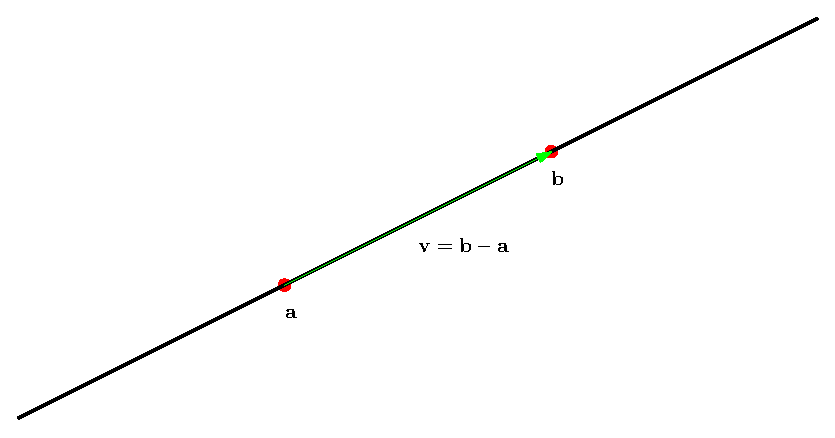
\includegraphics[width=0.85\textwidth]{img/line}
  \caption{Line identified by two points. See Equation~\ref{eq:line} }
  \label{fig:line}
\end{figure}

The Figure~\ref{fig:line} shows the line from Equation~\ref{eq:line} indentified by the points $\mathbf{a}$ and $\mathbf{b}$.
On these conditions; we can give continuos values to the parameter $s$ in the Equation~\ref{eq:line}, to obtain points on the line $\mathbf{L}$.
Particulary, if we let $s = 0$ we get the point $\mathbf{a}$ and if we let $s = 1$ we get  
$\mathbf{b}$.
Moreover, any value $0 \leq s \leq 1$ will get us a point $\mathbf{p}$ inside the line segment $\overline{\mathbf{a} \mathbf{b}}$.
Any value $s > 1$ will get a $\mathbf{p} \in \mathbf{L}$, $\mathbf{p} \notin \overline{\mathbf{a} \mathbf{b}}$ that is closer to $\mathbf{b}$ than it is to to $\mathbf{a}$.
Conversely, any $s < 0$ will get a $\mathbf{p} \in \mathbf{L}$, $\mathbf{p} \notin \overline{\mathbf{a} \mathbf{b}}$ that is closer to $\mathbf{a}$ than it is to $\mathbf{b}$.

We can use this last observations to identify segments and rays.
A \emph{ray} from $\mathbf{a}$ in the direction of $\mathbf{b}$ is the one that has Equation~\ref{eq:line}, with the constrain that the parameter must be $s > 0$.
The line \emph{segment} from $\mathbf{a}$ to $\mathbf{b}$, denoted by $\overline{\mathbf{a} \mathbf{b}}$, is the one that also follows Equation~\ref{eq:line}, with the constrain that   $0 \leq s \leq 1$.

\subsection{Point to line distance}

Given a line $\mathbf{L}$ and a point $\mathbf{p}$, we want to identify the distant $d$ from $\mathbf{p}$ to $\mathbf{L}$.
It's clear that if $\mathbf{p} \in \mathbf{L}$, then $d = 0$.
Now, if $\mathbf{p} \notin \mathbf{L}$, we want the distant between $\mathbf{p}$ and a certain point $\mathbf{q}$, such that $\mathbf{q} \in \mathbf{L}$ and $d(\mathbf{q}, \mathbf{p})$ is the minimal to all other points in $\mathbf{L}$.



\subsubsection{Point to segment distance}
\subsection{Ray to segment intersection}
\subsection{Belonging test on simple polygons}

